%\documentclass[dvipdfmx]{beamer}      % platex の場合
\documentclass{beamer}                 % lualatex の場合
\usepackage{mySld}

\begin{document}
\title{オペレーティングシステムの機能を使ってみよう\\
第4章 ファイルシステム}
\date{}

%===============================================================
\begin{frame}
  \titlepage
\end{frame}

%===============================================================
%\begin{frame}[fragile]
%  \frametitle{}
%\end{frame}

\section{ファイルシステム}
%===============================================================
\begin{frame}[fragile]
  \frametitle{ファイルシステム}
  \begin{itemize}
    \item \emph{ファイル}\\
      二次記憶装置に格納された不揮発性のデータ記憶のこと\\
      (二次記憶:HDD,USBメモリ,CD-ROM,SSD,…)
    \item \emph{ファイルシステム}\\
      二次記憶装置に多数のファイルを記憶・管理する仕組み\\
      記憶・管理されているファイルの集合
    \item \emph{UNIXファイルシステム}\\
      Windows や macOS のファイルシステムも基本は同じ
  \end{itemize}
\end{frame}

%===============================================================
\begin{frame}[fragile]
  \frametitle{ファイル木}
  \fig{scale=0.7}{FileSystem-crop.pdf}

  \begin{itemize}
  \item ルートディレクトリを根にした有向の木構造
  \item 節点(ノード)はディレクトリ(フォルダ)
  \item 葉(リーフ)はファイル
  \item 有向枝(エッジ)はリンク
  \item \emph{ファイルとリンクは独立している}
  \item ディレクトリもファイルの一種
  \end{itemize}
\end{frame}

%===============================================================
\begin{frame}[fragile]
  \frametitle{特別なディレクトリ}
  \fig{scale=0.8}{FileSystem2-crop.pdf}

  \begin{itemize}
  \item ルートディレクトリ(ファイル木の根になるディレクトリ)
  \item 親ディレクトリ(ルートに近いディレクリ,「\texttt{..}」で表す)
  \item カレントディレクトリ(現在位置,「\texttt{.}」で表す)
  \item ホームディレクトリ(ログイン時のカレントディレクトリ)
  \end{itemize}
\end{frame}

%===============================================================
\begin{frame}[fragile]
  \frametitle{パス(Path)}
  \begin{itemize}
  \item パスは径の意味(ファイルへの道)
  \item ファイルをパスにより特定できる.
  \item ファイル木のリンクに付いた名前を「\texttt{/}」で区切って書く.
  \item パスには以下の二種類がある.
    \begin{enumerate}
    \item[1] \emph{絶対パス} \\
      ルートディレクトリを起点にしたパス\\
      「\texttt{/}」で書き始める.\\
      例:\texttt{/home/mura/hello.c}
    \item[2] \emph{相対パス} \\
      カレントディレクトリを起点にしたパス
      「\texttt{/}」以外で書き始める.\\
      例:\texttt{hello.c}
    \end{enumerate}
  \end{itemize}
\end{frame}

%===============================================================
\begin{frame}[fragile]
  \frametitle{絶対パス}
  \fig{scale=0.7}{FileSystem-crop.pdf}

  ルートディレクトリを起点にしたパス
  \begin{itemize}
  \item \texttt{/etc/passwd}
  \item \texttt{/bin/ls}
  \item \texttt{/home/mura} : ディレクトリへのパス
  \item \texttt{/home/mura/hello.c}
  \item \texttt{/home/sige/../mura/./hello.c}
  \end{itemize}
\end{frame}

%===============================================================
\begin{frame}[fragile]
  \frametitle{相対パス}
  \fig{scale=0.7}{FileSystem-crop.pdf}

  カレントディレクトリを起点にしたパス\\
  (カレントディレクトリが\texttt{/home}のとき)
  \begin{itemize}
  \item \texttt{mura/hello.c}
  \item \texttt{sige} : ディレクトリへのパス
  \item \texttt{../bin/ls}
  \item \texttt{sige/../mura/hello.c}
  \end{itemize}
\end{frame}

%===============================================================
\begin{frame}[fragile]
  \frametitle{カレントディレクトリ}

  プロセス毎にカレント(現在の)ディレクトリがある.
  \begin{itemize}
  \item カレントディレクトリの変更は他のプロセスに影響はない.
  \item 他のターミナル(ターミナルもプロセス)に影響はない.
  \item 次回のログインにも引継がれない.
  \item 以下のコマンドで変更と確認ができる.
    \begin{itemize}
      \item \emph{変更(cd コマンド)} \\
        \texttt{ \$ cd パス }
      \item \emph{確認(pwd コマンド)} \\
        \texttt{ \$ pwd }
    \end{itemize}
  \end{itemize}
\end{frame}

%===============================================================
\begin{frame}[fragile]
  \frametitle{cd,pwdコマンドの実行例}

  \begin{minipage}{0.4\columnwidth}
%    \rightline{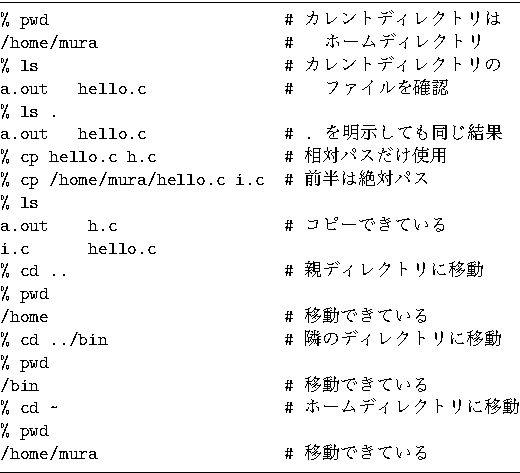
\includegraphics[viewport=0 0 130 225,clip=true]{../Fig/cdpwd.pdf}}
    \fig{viewport=0 0 130 225,clip=true}{cdpwd.pdf}
  \end{minipage}
  \begin{minipage}{0.55\columnwidth}
    \fig{scale=0.75}{FileSystem-crop.pdf}
  \end{minipage}
\end{frame}

%===============================================================
\begin{frame}[fragile]
  \frametitle{リンク(ハードリンク)}
  \fig{scale=0.8}{Link-crop.pdf}
  \begin{itemize}
  \item ファイルに別名を付ける.
  \item ハードリンクとシンボリックリンクの二種類がある.
  \item \emph{ハードリンク}
    \begin{itemize}
    \item 従来のリンクと同じもの
    \item 一つのファイル本体に複数のリンクが可能
    \item 元々あったリンク,後で追加したリンクに区別はない
    \end{itemize}
  \end{itemize}
\end{frame}

%===============================================================
\begin{frame}[fragile]
  \frametitle{リンク(ハードリンクの作成)}
  \fig{scale=0.8}{Link-crop.pdf}
  \emph{ln コマンドを用いる.}
  \centerline{
    \begin{minipage}{0.8\columnwidth}
      \lst{numbers=none}{ln.txt}
    \end{minipage}
  }
\end{frame}

%===============================================================
\begin{frame}[fragile]
  \frametitle{リンク(ハードリンクの削除)}
  \fig{scale=0.8}{Link-crop.pdf}
  \emph{rm コマンドを用いる.}
  \centerline{
    \begin{minipage}{0.8\columnwidth}
      \lst{numbers=none}{lnrm.txt}
    \end{minipage}
  }
\end{frame}

%===============================================================
\begin{frame}[fragile]
  \frametitle{リンク(シンボリックリンク)}
  \fig{scale=0.8}{SymLink-crop.pdf}
  \begin{itemize}
  \item \emph{シンボリックリンク}
    \begin{itemize}
    \item パスを格納した特殊なファイル
    \item ソフトリンクとも呼ぶ
    \item パス名の解釈時に字面で評価される
    \item 字面での評価なので制約が少ない(別ディスク,リンク切)
    \item ファイルが置換わると新しいファイルを参照する
    \end{itemize}
  \end{itemize}
\end{frame}

%===============================================================
\begin{frame}[fragile]
  \frametitle{リンク(シンボリックリンクの作成)}
  \fig{scale=0.8}{SymLink-crop.pdf}
  \emph{ln -s コマンドを用いる.}
  \centerline{
    \begin{minipage}{0.8\columnwidth}
      \lst{numbers=none}{lns.txt}
    \end{minipage}
  }
\end{frame}

%===============================================================
\begin{frame}[fragile]
  \frametitle{リンク(シンボリックリンクの削除)}
  \fig{scale=0.8}{SymLink-crop.pdf}
  \emph{rm コマンドを用いる.}
  \centerline{
    \begin{minipage}{0.8\columnwidth}
      \lst{numbers=none}{lnsrm.txt}
    \end{minipage}
  }
\end{frame}

%===============================================================
\begin{frame}[fragile]
  \frametitle{ファイルの属性}
  \emph{主な属性}
  \begin{description}
  \item[種類] 普通ファイル,ディレクトリ,シンボリックリンク等
  \item[保護モード] openシステムコールで紹介した\texttt{rwxrwxrwx}.
  \item[リンク数] ファイルを指しているハードリンクの数.
    リンク数が0になるとファイル本体が削除される.
    (例えば,ハードリンク例の\texttt{hello.c}ファイルの場合は3になる)
  \item[所有者] 所有者のユーザ番号.
  \item[グループ] 属するグループのグループ番号.
  \item[ファイルサイズ] ファイルの大きさ(バイト単位).
  \item[最終参照日時] 最後にアクセスした時刻.
  \item[最終変更日時] 内容を最後に変更した時刻.
  \item[最終属性変更時刻] 属性を最後に変更した時刻.
  \end{description}
\end{frame}

%===============================================================
\begin{frame}[fragile]
  \frametitle{属性の表示方法}
  \emph{ls -l コマンドを用いる.}
  \begin{lstlisting}[numbers=none]
$ ls -l a.txt
-rw-r--r--  1 mura  staff 10 May  1 18:18 a.txt
  \end{lstlisting}
\begin{description}
\item[ファイルの種類] 一文字目の「\texttt{-}」は
ファイルが普通のファイルであることを表している.
一文字目が「\texttt{d}」はディレクトリであること,
「\texttt{l}」はシンボリックリンクであることを表す.
\item[ファイルの保護モード] openシステムコールで紹介したもの
(\texttt{rwxrwxrwx}).
\item[リンク数] \texttt{1}はリンク数が1であることを表している.
\item[所有者] \texttt{mura}は
ファイルの所有者がユーザ mura であることを表している.
メタ情報の内部表現はユーザ番号であるが,
ls コマンドがユーザ名に変換して表示している.
\end{description}
\end{frame}

%===============================================================
\begin{frame}[fragile]
  \frametitle{属性の表示方法}
  \emph{ls -l コマンドを用いる.}
  \begin{lstlisting}[numbers=none]
$ ls -l a.txt
-rw-r--r--  1 mura  staff 10 May  1 18:18 a.txt
  \end{lstlisting}
\begin{description}
\item[グループ] \texttt{staff}は
ファイルがグループ staff に属することを表している.
メタ情報の内部表現はグループ番号であるが,
ls コマンドがグループ名に変換して表示している.
\item[ファイルサイズ] \texttt{10}はファイルのサイズが10バイトで
あることを表している.
\item[最終変更日時] \texttt{May 1 18:18} はファイルの最終変更日時である.
\item[パス] \texttt{a.txt} はファイルへ到達するために使用したパスである.
\emph{パス名(ファイル名)はファイルの属性ではない.}
\end{description}
\end{frame}

%===============================================================
\begin{frame}[fragile]
  \frametitle{属性の変更方法}
  \emph{chmod コマンドを用いる.}\\
  \begin{minipage}{0.48\columnwidth}
  \begin{lstlisting}[numbers=none]
$ chmod OOO ファイル...      # 書式1
$ chmod ugo+rwx ファイル...  # 書式2
$ chmod ugo-rwx ファイル...  # 書式3
  \end{lstlisting}
  \end{minipage}
  \begin{minipage}{0.48\columnwidth}
  \tbl{scale=0.8}{chmodOptions.pdf}
  \end{minipage}

\begin{description}
\item[書式1] \texttt{OOO}は3桁の8進数である.
8進数で保護モードを指定する.
8進数の値のはopenシステムコールの書式2と同じである.

\item[書式2,3] \texttt{ugo+-rwx}の文字を組合せて
保護モードの変更方法を記述する.
各文字の意味は上の通りである。
例えば,
所有者とグループに書込み権と実行権を与える場合なら\texttt{ug+wx}のように書く.
その他のユーザの読出し権を取上げるなら\texttt{o-r}のように書く.
\end{description}
\end{frame}

%===============================================================
\begin{frame}[fragile]
  \frametitle{属性の変更方法}
  \emph{chmod コマンドの使用例}
  \centerline{
    \begin{minipage}{0.8\columnwidth}
      \lst{numbers=none}{chmod.txt}
    \end{minipage}
  }
\end{frame}

%===============================================================
\begin{frame}[fragile]
  \frametitle{課題 No.3(1/4)}
  \emph{1. パスとハードリンク}
\begin{enumerate}
\item[(a)] 自分のホームディレクトリのパスを調べる.
\item[(b)] ハードリンクに関する課題を行うために,
ディレクトリ\texttt{/tmp}にカレントディレクトリを移動する\footnote{
PC教室のMacはユーザのホームディレクトリを共有ドライブ上に置いている.
\texttt{/tmp}はローカルハードディスク上にある.}.
\item[(c)] \texttt{/tmp}以下に図のディレクトリやファイルを作る.
\item[(d)] \texttt{ls -l}を用いてファイルの種類やリンク数を確認する.
\end{enumerate}

\fig{scale=0.7}{Link-crop.pdf}
\end{frame}

%===============================================================
\begin{frame}[fragile]
  \frametitle{課題 No.3 (2/4)}
\begin{enumerate}
\item[(e)] 相対パスを用いて\texttt{hello.c}の内容を表示する.\\
(表示には\texttt{cat}コマンドを用いると良い.)
\item[(f)] 絶対パスを用いて\texttt{hello.c}の内容を表示する.
\item[(g)] \texttt{h1.c}を利用した相対パスを用いて
\texttt{hello.c}の内容を表示する.
\item[(h)] \texttt{ex1.c}を利用した相対パスを用いて
\texttt{hello.c}の内容を表示する.
\item[(i)] カレントディレクトリを\texttt{SysPro}に変更する.
\item[(j)] \texttt{ex1.c}を利用した相対パスを用いて
\texttt{hello.c}の内容を表示する.
\item[(k)] \texttt{hello.c}を利用した相対パスを用いて
\texttt{hello.c}の内容を表示する.
\item[(l)] ディレクトリのハードリンクができるか試す.
\item[(m)] 課題のために作成したファイルやディレクトリを全て削除する.
\end{enumerate}
\end{frame}

%===============================================================
\begin{frame}[fragile]
  \frametitle{課題 No.3 (3/4)}
  \emph{2. シンボリックリンク}
\begin{enumerate}
\item[(a)] シンボリックリンクを作ってみる.
\item[(b)] シンボリックリンクを\texttt{ls -l}を用いて確認する.
\item[(c)] シンボリックリンクを用いてファイルをアクセスできることを確認する.
\item[(d)] リンク切れのシンボリックリンクを使用するとどうなるか確認する.
\item[(e)] ディレクトリに対するリンクを作って使用できることを確認する.
\item[(f)] 他のディレクトリにあるファイルをリンクして使用できることを確認する.
\item[(g)] シンボリックリンクのループを作る.(a.txt →  b.txt,b.txt →  a.txt)
\item[(h)] ループしているシンボリックリンクを使用するとどうなるか確認する.
(\|$ cat a.txt|)
\end{enumerate}
\end{frame}

%===============================================================
\begin{frame}[fragile]
  \frametitle{課題 No.3 (4/4)}
  \emph{3. 保護モード}
\begin{enumerate}
\item[(a)] テキストファイル(\texttt{hello.c})と
実行可能ファイル(\texttt{a.out})を準備する.
\item[(b)] \texttt{chmod}で保護モードを変化させてみる.
\item[(c)] \texttt{ls -l}で変化を確認する.
\item[(d)] 保護モードを変化させて,ファイルの読出しや実行ができるか確認する.
\item[(e)] ディレクトリの保護モードは何の意味を持つか考える.
\end{enumerate}
\end{frame}

\end{document}
